El estudio de series temporales ofrece una perspectiva din�mica de cualquier sistema. En concreto, analizar el microbioma humano a lo largo del tiempo nos permite dilucidar el comportamiento de las bacterias que viven con nosotros, las cuales influyen directamente en la salud humana. En este estudio se demuestra que en condiciones normales, el microbioma tiene cierta estabilidad. Sin embargo, cuando el hospedador cambia de ambiente realizando un viaje al extranjero, su flora intestinal se desequilibra debido a la nueva dieta y el tipo de agua del lugar de destino. Este suceso hace que aparezcan nuevos g�neros y desaparezcan otros existentes. Cuando el sujeto regresa a su pa�s de origen y a sus h�bitos cotidianos, el microbioma recupera la estabilidad inicial. Tambi�n se ha analizado la micobiota de la cavidad oral pero �sta no sufre tanto la perturbaci�n como el intestino.

Una cuesti�n interesante que surge de este estudio es, �qu� le pasa al microbioma de una persona emigrante? Si el sujeto hubiera permanecido m�s tiempo en el extranjero hubiera sido muy interesante comprobar lo que sucede. Algunas posibilidades pueden ser (i) que alcance un nuevo estado de equilibrio, ya sea uno igual al estado inicial o uno nuevo (lo que ser�a interesante poder demostrar cu�nto tiempo se necesita para adquirir el equilibrio) y (ii) que nunca alcance el estado de equilibrio (lo cual ser�a poco probable ya que no existen casos de diarrea cr�nica causadas por un viaje). La hip�tesis m�s probable es que la primera porque la variabilidad disminuye de forma exponencial a partir del d�a 100, de lo que se deduce que ya hab�a alcanzado el equilibrio antes de su regreso. Otra cuesti�n interesante es �por qu� no hay un nuevo desequilibrio a la vuelta del viaje? El microbioma parece que tiene memoria y no sufre tanto al exponerse a un ambiente que ya le es conocido.

En este proyecto tambi�n se ha estudiado lo que ocurre en el caso de que un sujeto tenga una infecci�n intestinal causada por un pat�geno. De nuevo, la estabilidad de su microbioma se rompe y se puede medir el tiempo que tarda en recuperarse. Se demuestra que una infecci�n supone el cambio del microbioma a un equilibrio nuevo. Este mismo efecto ocurre con la ingesta de antibi�ticos, que afecta a la mayor�a de microorganismos y los oportunistas ocupan esos nichos conformando un nuevo equilibrio.

La aplicaci�n de este tipo de estudios radica en monitorizar la administraci�n de probi�ticos para prevenir y tratar enfermedades como la obesidad o la diabetes. Se requiere de forma paralela un an�lisis metabol�mico para conocer la composici�n funcional de la flora intestinal y el estado inmunol�gico del hospedador. Con estas investigaciones, se pueden dilucidar los mecanismos moleculares del microbioma que influyen en las enfermedades y har� posible adoptar un nuevo enfoque en el desarrollo de terapias aprovechando los beneficios de la modulaci�n de la microbiota intestinal sobre el metabolismo.

Para alcanzar esa meta a�n queda un largo camino que recorrer. Los trabajos hasta la fecha han supuesto un enorme avance y adem�s se ha logrado en un periodo de tiempo relativamente corto. Como ya se ha comentado, tanto las tecnolog�as de secuenciaci�n como los sistemas de clasificaci�n no son perfectos todav�a e introducen errores en los resultados. Adem�s, se ha demostrado que los intentos de explicar las relaciones entre microorganismos mediante correlaciones no muestran las verdaderas interacciones \cite{Fisher2014}. En ese mismo art�culo, los autores proponen una aproximaci�n capaz de superar todos esos obst�culos a la que han llamado LIMITS (detallada en Materiales y m�todos). Para comprobar su potencial y comparar los resultados expuestos en apartados anteriores, se aplic� LIMITS a los datos del estudio. En la figura \ref{LIMITS_salivaA} se puede observar un ejemplo que compara la matriz de correlaciones de saliva A con la matriz de interacciones propuesta por LIMITS para saliva A.

\begin{figure}[!h]
    \centering    
    \subfigure{
    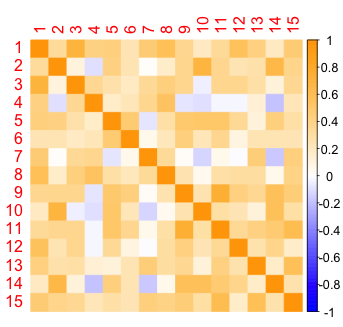
\includegraphics[width=4.5in]{./Figuras/corrplot_salivaA_formatLIMITS.png}}
    \subfigure{
    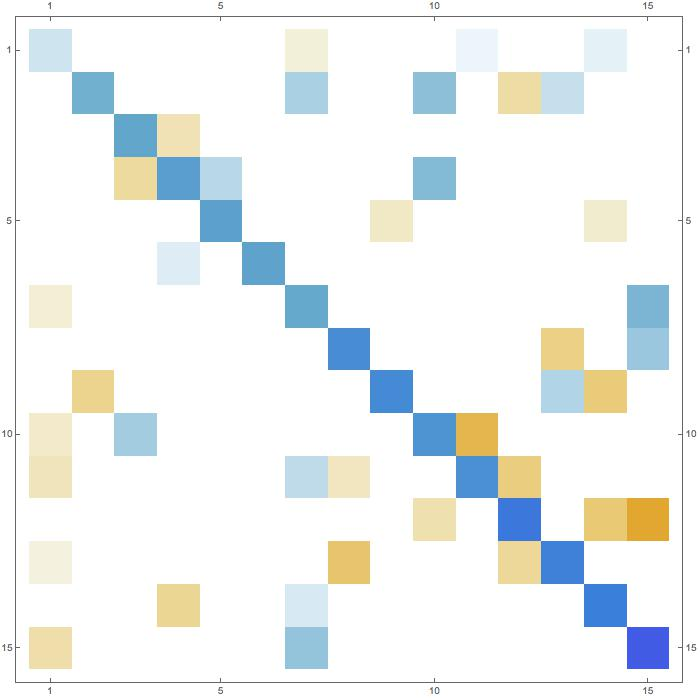
\includegraphics[width=4.5in]{./Figuras/SalivaA_15otus_alltimes.jpg}}
    \caption{Correlaci�n Pearson vs. LIMITS en saliva A}
    \label{LIMITS_salivaA}
\end{figure}

